\documentclass{beamer}
\usetheme{Madrid} % Clean theme
\usepackage{listings}
\usepackage{xcolor}
\usepackage{graphicx}

% Code listing style
\lstset{
  basicstyle=\ttfamily\footnotesize,
  keywordstyle=\color{blue},
  stringstyle=\color{orange},
  commentstyle=\color{green!60!black},
  breaklines=true,
  frame=single,
  showstringspaces=false
}

\title{MatGeo Assignment - Problem 1.5.12}
\author{EE25BTECH11024}
\institute{IIT Hyderabad}
\date{\today}

\begin{document}

% Title slide
\begin{frame}
  \titlepage
\end{frame}

% Problem statement
\begin{frame}{Problem Statement}
In what ratio does the point $P(-4, y)$ divide the line segment joining 
$A(-6,10)$ and $B(3,-8)$? Hence, find the value of $y$.
\end{frame}

% Solution
\begin{frame}{Solution}
Using the section formula:
\[
x = \frac{mx_2 + nx_1}{m+n}, \quad 
y = \frac{my_2 + ny_1}{m+n}
\]

Substitute $x = -4$, $A(-6,10)$, $B(3,-8)$:

\[
-4 = \frac{3m - 6n}{m+n} \implies m:n = 2:7
\]

\[
y = \frac{2(-8) + 7(10)}{9} = 6
\]

\textbf{Answer:} Ratio $2:7$, and $y=6$.
\end{frame}

\begin{frame}{Resulting Graph}
\centering
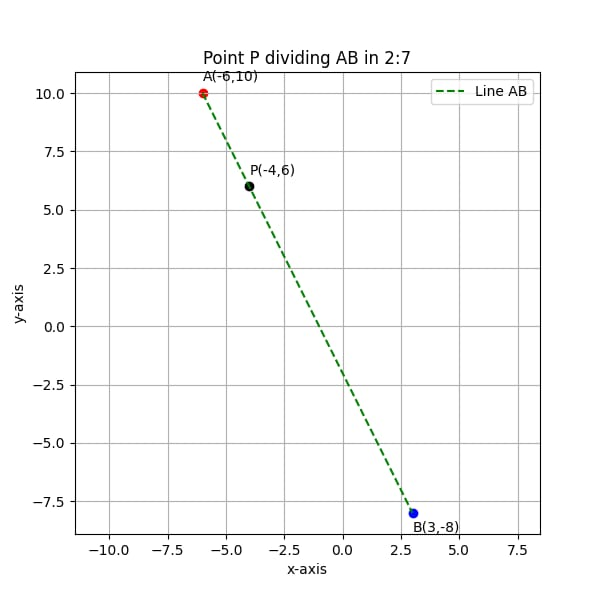
\includegraphics[width=0.6\linewidth]{figs/fig.jpg}
\end{frame}

% Python code 1
\begin{frame}[fragile]{Python Code: plot.py (Native)}
\begin{lstlisting}[language=Python]
import numpy as np
import matplotlib.pyplot as plt

# Given points
A = np.array([-6, 10])
B = np.array([3, -8])
P = np.array([-4, 6])   # Found from calculation

# Plotting
plt.figure(figsize=(6,6))
plt.plot([A[0], B[0]], [A[1], B[1]], 'g--', label="Line AB")
plt.scatter(*A, color="red")
plt.scatter(*B, color="blue")
plt.scatter(*P, color="black")

# Labels
plt.text(A[0], A[1]+0.5, "A(-6,10)", fontsize=10)
plt.text(B[0], B[1]-0.8, "B(3,-8)", fontsize=10)
plt.text(P[0], P[1]+0.5, "P(-4,6)", fontsize=10)
\end{lstlisting}
\end{frame}


\begin{frame}[fragile]{Python Code (Native Implementation – plot.py)}
\begin{lstlisting}[language=Python]
plt.xlabel("x-axis")
plt.ylabel("y-axis")
plt.title("Point P dividing AB in 2:7")
plt.legend()
plt.grid(True)
plt.axis("equal")
plt.show()
\end{lstlisting}
\end{frame}

\begin{frame}[fragile]{C Code (Shared Library – find_point.c)}
\begin{lstlisting}[language=C]
#include <stdio.h>

void find_point(double *px, double *py) {
    // A(-6,10), B(3,-8)
    double x1 = -6, y1 = 10, x2 = 3, y2 = -8;
    int m = 2, n = 7; // ratio

    *px = (m*x2 + n*x1) / (m+n);
    *py = (m*y2 + n*y1) / (m+n);
}
\end{lstlisting}
\end{frame}

% Python code 2
\begin{frame}[fragile]{Python Code: call.py (C + Python)}
\begin{lstlisting}[language=Python]
import ctypes
import numpy as np
import matplotlib.pyplot as plt

# Load shared object
so = ctypes.CDLL("./find_point.so")

# Prepare arguments
px = ctypes.c_double()
py = ctypes.c_double()

so.find_point(ctypes.byref(px), ctypes.byref(py))

A = np.array([-6, 10])
B = np.array([3, -8])
P = np.array([px.value, py.value])

# Plot
plt.figure(figsize=(6,6))
plt.plot([A[0], B[0]], [A[1], B[1]], 'g--', label="Line AB")
\end{lstlisting}
\end{frame}

\begin{frame}[fragile]{Python Code (C Integrated – call.py)
}
\begin{lstlisting}[language=Python]
plt.scatter(*A, color="red")
plt.scatter(*B, color="blue")
plt.scatter(*P, color="black")

plt.text(A[0], A[1]+0.5, "A(-6,10)", fontsize=10)
plt.text(B[0], B[1]-0.8, "B(3,-8)", fontsize=10)
plt.text(P[0], P[1]+0.5, f"P({px.value:.1f},{py.value:.1f})", fontsize=10)

plt.xlabel("x-axis")
plt.ylabel("y-axis")
plt.title("Point P from C code")
plt.legend()
plt.grid(True)
plt.axis("equal")
plt.show()
\end{lstlisting}
\end{frame}



\end{document}
